\documentclass[12pt]{article}
\usepackage{bbold}
\usepackage{amsfonts}
\usepackage{amsmath}
\usepackage{amssymb}
\usepackage{color}
\setlength{\columnseprule}{1pt}
\usepackage[utf8]{inputenc}
\usepackage[T2A]{fontenc}
\usepackage[english, russian]{babel}
\usepackage{graphicx}
\usepackage{hyperref}
\usepackage{mathdots}
\usepackage{xfrac}


\def\columnseprulecolor{\color{black}}

\graphicspath{ {./resources/} }


\usepackage{listings}
\usepackage{xcolor}
\definecolor{codegreen}{rgb}{0,0.6,0}
\definecolor{codegray}{rgb}{0.5,0.5,0.5}
\definecolor{codepurple}{rgb}{0.58,0,0.82}
\definecolor{backcolour}{rgb}{0.95,0.95,0.92}
\lstdefinestyle{mystyle}{
    backgroundcolor=\color{backcolour},   
    commentstyle=\color{codegreen},
    keywordstyle=\color{magenta},
    numberstyle=\tiny\color{codegray},
    stringstyle=\color{codepurple},
    basicstyle=\ttfamily\footnotesize,
    breakatwhitespace=false,         
    breaklines=true,                 
    captionpos=b,                    
    keepspaces=true,                 
    numbers=left,                    
    numbersep=5pt,                  
    showspaces=false,                
    showstringspaces=false,
    showtabs=false,                  
    tabsize=2
}

\lstset{extendedchars=\true}
\lstset{style=mystyle}

\newcommand\0{\mathbb{0}}
\newcommand{\eps}{\varepsilon}
\newcommand\overdot{\overset{\bullet}}
\DeclareMathOperator{\sign}{sign}
\DeclareMathOperator{\re}{Re}
\DeclareMathOperator{\im}{Im}
\DeclareMathOperator{\Arg}{Arg}
\DeclareMathOperator{\const}{const}
\DeclareMathOperator{\rg}{rg}
\DeclareMathOperator{\Span}{span}
\DeclareMathOperator{\alt}{alt}
\DeclareMathOperator{\Sim}{sim}
\DeclareMathOperator{\inv}{inv}
\DeclareMathOperator{\dist}{dist}
\newcommand\1{\mathbb{1}}
\newcommand\ul{\underline}
\renewcommand{\bf}{\textbf}
\renewcommand{\it}{\textit}
\newcommand\vect{\overrightarrow}
\newcommand{\nm}{\operatorname}
\DeclareMathOperator{\df}{d}
\DeclareMathOperator{\tr}{tr}
\newcommand{\bb}{\mathbb}
\newcommand{\lan}{\langle}
\newcommand{\ran}{\rangle}
\newcommand{\an}[2]{\lan #1, #2 \ran}
\newcommand{\fall}{\forall\,}
\newcommand{\ex}{\exists\,}
\newcommand{\lto}{\leftarrow}
\newcommand{\xlto}{\xleftarrow}
\newcommand{\rto}{\rightarrow}
\newcommand{\xrto}{\xrightarrow}
\newcommand{\uto}{\uparrow}
\newcommand{\dto}{\downarrow}
\newcommand{\lrto}{\leftrightarrow}
\newcommand{\llto}{\leftleftarrows}
\newcommand{\rrto}{\rightrightarrows}
\newcommand{\Lto}{\Leftarrow}
\newcommand{\Rto}{\Rightarrow}
\newcommand{\Uto}{\Uparrow}
\newcommand{\Dto}{\Downarrow}
\newcommand{\LRto}{\Leftrightarrow}
\newcommand{\Rset}{\bb{R}}
\newcommand{\Rex}{\overline{\bb{R}}}
\newcommand{\Cset}{\bb{C}}
\newcommand{\Nset}{\bb{N}}
\newcommand{\Qset}{\bb{Q}}
\newcommand{\Zset}{\bb{Z}}
\newcommand{\Bset}{\bb{B}}
\renewcommand{\ker}{\nm{Ker}}
\renewcommand{\span}{\nm{span}}
\newcommand{\Def}{\nm{def}}
\newcommand{\mc}{\mathcal}
\newcommand{\mcA}{\mc{A}}
\newcommand{\mcB}{\mc{B}}
\newcommand{\mcC}{\mc{C}}
\newcommand{\mcD}{\mc{D}}
\newcommand{\mcJ}{\mc{J}}
\newcommand{\mcT}{\mc{T}}
\newcommand{\us}{\underset}
\newcommand{\os}{\overset}
\newcommand{\ol}{\overline}
\newcommand{\ot}{\widetilde}
\newcommand{\vl}{\Biggr|}
\newcommand{\ub}[2]{\underbrace{#2}_{#1}}

\def\letus{%
    \mathord{\setbox0=\hbox{$\exists$}%
             \hbox{\kern 0.125\wd0%
                   \vbox to \ht0{%
                      \hrule width 0.75\wd0%
                      \vfill%
                      \hrule width 0.75\wd0}%
                   \vrule height \ht0%
                   \kern 0.125\wd0}%
           }%
}
\DeclareMathOperator*\dlim{\underline{lim}}
\DeclareMathOperator*\ulim{\overline{lim}}

\everymath{\displaystyle}

% Grath
\usepackage{tikz}
\usetikzlibrary{positioning}
\usetikzlibrary{decorations.pathmorphing}
\tikzset{snake/.style={decorate, decoration=snake}}
\tikzset{node/.style={circle, draw=black!60, fill=white!5, very thick, minimum size=7mm}}

\title{Архитектура ЭВМ. Теория}
\author{Александр Сергеев}
\date{}

\begin{document}
\maketitle
\section{Представление чисел}
\subsection{Представление целых чисел}
\textbf{Определение}\\
\textit{Байт} - минимальная адресуемая ячейка памяти.\\\\
Байт может быть не из 8 бит\\
Поэтому в сетевых протоколах - \textit{аккет} - 8 бит.\\\\
Для беззнаковых чисел: бит - число в двоичной системе.\\
Для отрицательных чисел: \\
\begin{enumerate}
    \item Простая система\\
    Старший бит - под знак(0 - плюс, 1 - минус)\\
    \begin{itemize}
        \item[$(+)$] signed n>0 = unsigned n>0 (благодаря 0 - плюс)
        \item[$(-)$] +0 = 00000000, -0 = 11111111
    \end{itemize}
    \item Форма со сдвигом\\
    Храним число на сдвиг больше нашего.\\
    -128\ldots127/-127\ldots128 храним как 0\ldots255 (сдвиг на 128/127)\\\\
    \item Двоичный дополнительный код(система дополнения до 2)\\
    Веса битов:\\
    -128 64 32 16 8 4 2 1\\\\
    $-x = \overline{x}+1$
    \begin{itemize}
        \item[$(+)$] signed n>0 = unsigned n>0
        \item[$(+)$] сложение как у беззнаковой арифметики
        \item[$(-)$] Умножение и деление не аналогично беззнаковой арифметики
        \item[$(-)$] Фиксированное количество битов без возможности масштабирования(т.к. старший бит не подобен остальным)
    \end{itemize}
    \textit{Модулярная арифметика} - при выходы за границы берется значение по модулю.(плюсы: при временном выходе из диапазона можно вернуться)\\\\
    \textit{Арифметика с насыщением} - при выходы за границы берется максимум.\\\\
    \textit{Арифметика с генерацией ошибки} - при выходы за границы генерируется ошибка.\\
    \item Форма дополнения до 1\\
    Веса битов:\\
    -127 64 32 16 8 4 2 1
    \begin{itemize}
        \item[$(+)$] $-n = \overline{n}$
        \item[$(-)$] +0 = 00000000, -0 = 11111111
    \end{itemize}
    \item Код с чередованием\\
    Коды $0, 1, \ldots$ кодируют $0, -1, 1, -2, 2, \ldots$\\
    Получаем, что положительные числа $n$ кодируется как $n << 1$,\\
    а отрицательные $-n$ - как $((n-1) << 1) | 1$
    \begin{itemize}
        \item[$(+)$] Удобно для компактного хранения
        \item[$(-)$] Сложная арифметика
    \end{itemize}
    \item Отрицательное основание системы счисления\\
    Бит - цифра представления числа в системе счисления с основанием -2\\
    \begin{itemize}
        \item[$(+)$] Безболезненное добавление нулей слева(масштабируемость)
        \item[$(-)$] Чисел одного знака в 2 раза больше, чем другого
    \end{itemize}
    \item Симметричная троичная система\\
    Цифры -1(z), 0 ,1\\
    Веса разрядов $1, 3, 9, \ldots$.
    \begin{itemize}
        \item[$(+)$] $n \rightarrow -n \Leftrightarrow (z,0,1) \rightarrow (1,0,z)$
    \end{itemize}
    Перевод числа n:
    \begin{itemize}
        \item Если $|n-3^i| < |n|$, добавляем 1 в i-ый разряд, $n\,\text{–=}\,3^i$
        \item Если $|n+3^i| < |n|$, добавляем z в i-ый разряд, $n\,\text{+=}\,3^i$
    \end{itemize}
      
\end{enumerate}
int в C - хранит значения из диапазона не хуже, чем -32767..32767(во время создания C использовалась в том числе форма дополнения до 1, поэтому стандарт работает на форме дополнения и до 2, и до 1). \\Отсюда переполнение - undefined behaviour. Для беззнаковой арифметики - модулярная арифметика.
\subsection{Представление дробных чисел с фиксированной точкой}
\textit{Алгоритм перевода дробного числа в двоичную систему}\\
\begin{itemize}
    \item Часть до точки - как обычно
    \item Дробная часть - циклически берем целую часть от домножения на 2
\end{itemize}
\textit{Форма со сдвигом} - число n формата a.b(a бит для целой части, b бит для дробной) хранится в виде $n\cdot 2^b$.\\\\
(округление к ближайшему, иначе к четному)\\
Математика(для формата a.b):\\
\begin{itemize}
    \item Сложение/вычитание: $z=x+y$
    \item Умножение: $z=\frac{xy}{2^b}$
    \item Деление: $z=\frac{x}{y}\cdot 2^b$
\end{itemize}
Перевод числа $x$ в десятичное дробное число с $C$ знаками после запятой:
\begin{lstlisting}[language=C]
unsigned int y;
if (x < 0) {
    y = -(unsigned int)x;   //см. замечание
    printf("-");
} else {
    y = x;
}
printf("%u.", x / 0x10000);
x %= 0x10000;
printf("%02u", x * 1EC / 0x10000);
\end{lstlisting}
\textbf{Замечание}\\
Для x = INT\_MIN: x == -x, поэтому требуется беззнаковая переменная для хранения модуля x\\\\
Логический сдвиг направо - слева заполнение 0\\
Арифметический сдвиг направо - слева остается старший бит(деление на степень 2 с округлением к вниз\\
Арифметический сдвиг влево = Логический сдвиг влево - справа заполнение 0\\
Целочисленние деление - с окреглением к 0.
\subsection{Представление дробных чисел с плавающей точкой}
Числа в показательной форме(основание 10) - разложение числа на \textit{мантису} вида $\pm X,XXX\cdots$ и \textit{эксоненту} вида $10^{\pm XX\cdots X }$.\\
Стандарт \textit{IEEE-754}:\\
\begin{center}
    \begin{tabular}{|c|c|c|}
        \hline
        S & exp  & mant \\
        (бит знака) & (основание 2, & (без ведущей 1,\\
        & форма со сдвигом & заполняется без ведущих 0,\\
        & с округлением вниз) & округление к ближайшему, затем к четному)\\
        \hline
    \end{tabular}
\end{center}
Виды форматов
\begin{center}
    \begin{tabular}{c|c|c|c|c}
        всего,б & exp,б & mant,б & название & комментарий \\
        \hline
        16 & 5 & 10 & half &\\
        32 & 8 & 23 & single &\\
        64 & 11 & 52 & double &\\
        128 & 15 & 112 & quad & редко поддерживается железом(не в x86)\\
        \hline
        80 & 15 & 64 & extended & хранится ведущая единица, есть поддержка x86\\
        16 & 8 & 7 & bfloat & иногда поддерживается железом, удобно для нейронок
    \end{tabular}
\end{center}
\textbf{Замечание}:\\
Т.к. мантиса вида $0\ldots0$ является специальным случаем, мантиса хранит значения в диапазное $(0\ldots1)\ldots(1\ldots1)$. Тогда всего в мантисе хранится $2^n-1$ значений, где $n$ -длина мантисы. Тогда сдвиг будет $\left\lfloor\frac{2^n-1}2\right\rfloor$ = $2^{n-1}-1$\\
\textbf{Замечание}:\\
Т.к. показательная форма двоичного числа всегда начинается с 1, ее можно не хранить.\\\\
\textbf{Замечание}:\\
В Си \\float = single, \\double = double, \\long double = double/quad/extended\\\\
\begin{lstlisting}[language = C]
    x = 1.0000000000*2^(-14); //в формате half; в битовой форме 00000010000000000
    y = 1.0000000001*2^(-14); //в формате half; в битовой форме 00000010000000001
    x == y; //false
    y-x == 0; //true - проблема
\end{lstlisting}
Если экспонента заполнена 0:\\
\textit{Денормализованное число} - число вида $0.mant*2^{min}$, где $min$ - минимальная экспонента(исключая экспоненту $0\ldots0$), т.е. экспонента вида $0\ldots1$.\\
Обозначение экспоненты - нули в разделе экспонент.\\
Другими словами, если в разделе экспоненты нули, вместо подразумеваемой единицы у нас подразумеваемый 0, а сама экспонента равна $0000\ldots 0001$(учитывая формата со сдвигом).\\
Для half -- -14
Для single -- -126
Для double -- -1022
Для quad -- -16382
Такие числа позволяют расширить диапазон в сторону маленьких значений, добавить 0 в систему и решить пролему с вычитанием.\\
Переключение происходит автоматически в случае, если мы выходим из нормального диапазона.\\
В x86 есть поддержка, но с большими подениями скорости.\\\\
Если экспонента заполнена 1:
\begin{enumerate}
    \item Если мантиса == 0, то значения $\pm\infty$ в зависимости от бита знака
    \item Если мантиса != 0, то значение NaN
\end{enumerate}
Свойства NaN:
\begin{enumerate}
    \item Любые операции с NaN дают NaN
    \item NaN != NaN всегда true, остальные операции дают false
    \item Если старший бит мантисы - 1, считают(в стандарте не указано), что QNaN. При операции с ним исключения, если возможно
    \item Если младший бит мантисы - 0, считают(в стандарте не указано), что SNaN. Никаких исключений
\end{enumerate}
size\_t -- беззнаковый тип данных, который зависит от битности системы. В 32-битных системах size\_t имеет 32 бита, в 64-битных системах -- 64 бита.\\
\textbf{Алгоритм суммирования Кэхэна}
\begin{lstlisting}[language=C]
    double s = 0, c = 0;
    for (size_t i = 0; i < N; i++){
        double y = x[i] - c;
        double t = s + y;
        c = t - s - y;      //c - остаток от суммы, который отбрасывается при суммировании
        s = t;
    }
\end{lstlisting}
\section{Периферия}
\textit{Дребезг контактов} - явление, когда при нажатии на кнопку переключатель отскакивает от контакта, из-за чего возникают вспышки и затухания напряжения\\
Время колебаний зависит от изношенности и окисленности контактов\\
Решения: аппаратное или программное\\
Аппаратное - через RS-триггер и переключатель на два контакта, один - 0, второй - 1
\section{Логические операции}
Возьмем за базовые операции "НЕ", "И", "ИЛИ", "XOR".\\
Порядок операций: $\lnot, \land, \oplus, \lor$\\
\textit{Полусумматор(hsum)} - логический элемент, который принимает два однобитовых числа и возвращает бит суммы(xor) и бит переноса(and).\\
\textit{Мультиплексор} - по адресу на входе выдает один из входов на выход.\\
\textit{2to4Dec(2 к 4 декодер)} - по адресу на входе выдает единицу на данный выход.\\
\textit{RS-триггер(R = Reset, S = Set)} - элемент, который сохраняет значение при (R=S=0), обнуляет значение при (S=0, R=1) и записывает единицу при (S=1, R=0)(реализацию можно найти в интернете)\\
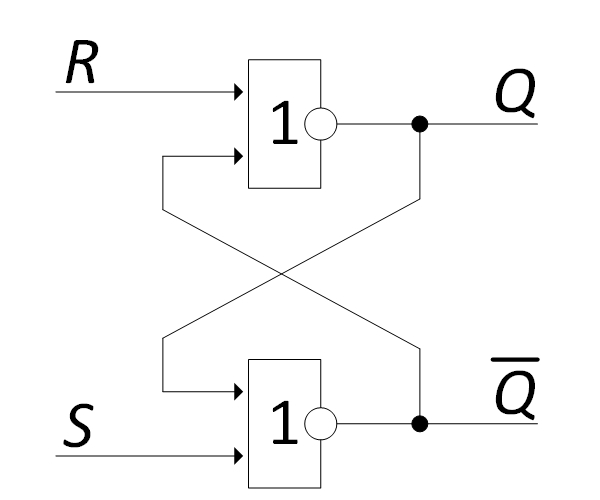
\includegraphics[height=5cm]{RS-trigger}\\\\
Некоторые проблемы электроники:
\begin{enumerate}
    \item За 1 такт при частоте 3ГГц свет пройдет расстояние не более 10 см(а электрон еще меньше)
    \item Из-за разной длины проводов одновременно выпущенные сигналы могут приходить с разной задержкой
    \item Провода обладают индуктивностью и могут передавать энергию друг другу, создавая помехи\\
    \textit{Оптика используется, чтобы избежать этой проблемы}
\end{enumerate}
\textit{Синхронизация}:
\begin{enumerate}
    \item Отправка сигналов происходит, пока на проводе синхронизации 0
    \item Выполнение операции происходит, когда на проводе 1
\end{enumerate}
\textit{Синхронный RS-триггер} - выполняет запись только по clock = 1\\
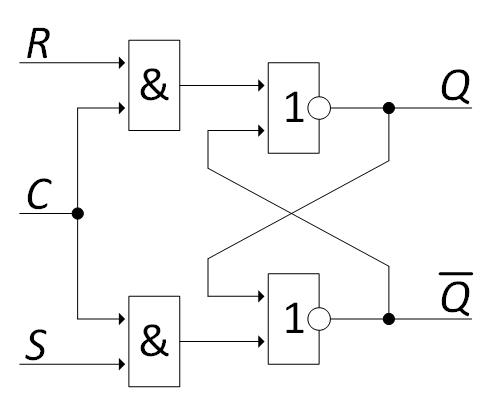
\includegraphics[height=5cm]{RS-trigger-sync}\\\\
\textit{Синхронный D-триггер} - триггер, который по clock = 1 записывает в триггер значение D, иначе сохраняет значение\\
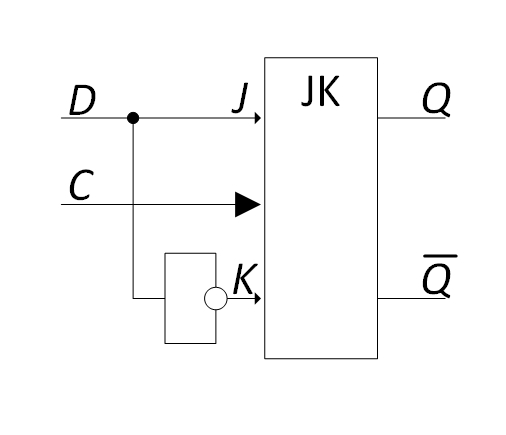
\includegraphics[height=5cm]{D-trigger}\\
\textit{(Вариант триггера на JK-триггере. Вариант на RS-триггере аналогичен)}\\\\
\textit{JK-триггер(J = Jump, K = Kill)} - элемент, который сохраняет значение при (J=K=0), обнуляет значение при (K=0, J=1), записывает единицу при (J=1, K=0) и инвертирует значение при (J=K=1).\\
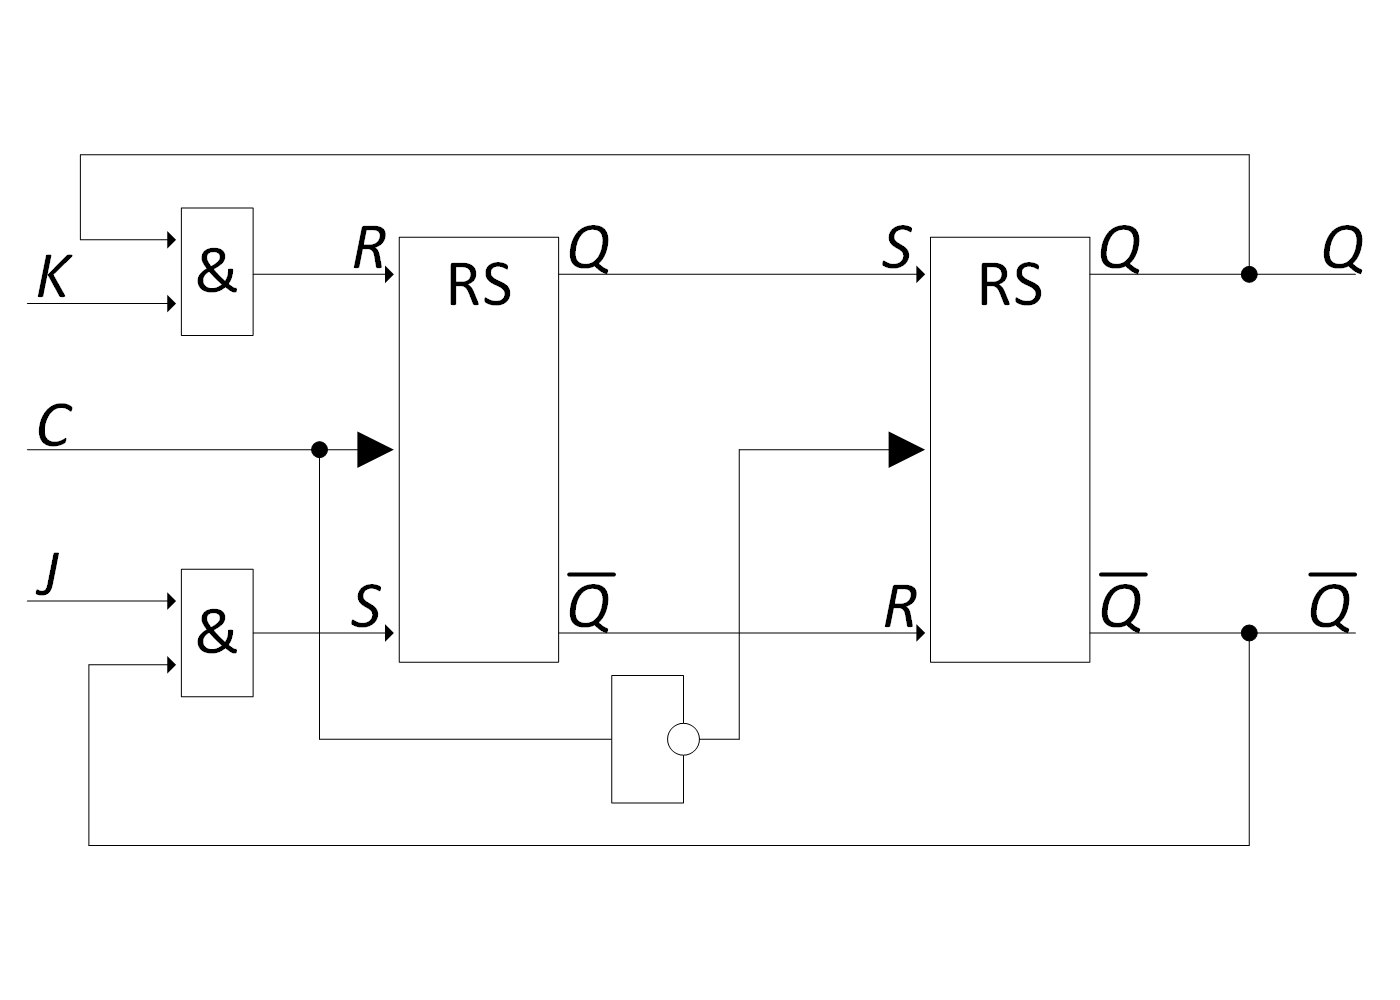
\includegraphics[height=5cm]{JK-trigger}\\\\
\subsection{Транзисторы}
В основном логические элементы строятся на транзисторах\\
Транзисторы
\begin{enumerate}
    \item Биполярные транзисторы(PNP/NPN)
    \item Полевые транзисторы\\
    Под действием положительного поля электроны в p-зоне поднимаются к подложке, становясь носителями заряда внутри кремниевой простойки(полевой транзистор с n-каналом, основанный на обогащении)\\
    Под действием отрицательного поля дырки в n-зоне поднимаются к подложке, становясь носителями заряда внутри кремниевой простойки(полевой транзистор с p-каналом)\\
    Иногда исток замыкают на подложку, чтобы она не создавала поле\\
    В таком случае при подключении транзистора обратной полярностью он становится диодом и пропускает ток\\
\end{enumerate}
\section{Память}
Память:
*TODO динамическая и статическая*
\begin{enumerate}
    \item Статическая память\\
    Используется в регистрах и кэше процессора
    Сигнал хранит состояние открытости транзистора
    \begin{enumerate}
        \item[-] Больше
        \item[-] Дороже
        \item[+] Считывание не разрушает данные
        \item[+] Транзистор переключается быстрее, а значит выше частота(из-за чего выше энергопотребление)
     \end{enumerate}
    \item Динамическая память\\
    Используется в RAM и иногда на последних уровнях кэш-памяти
    Сигнал хранит заряд транзистора
    \begin{enumerate}
        \item[+] Меньше
        \item[+] Дешевле
        \item[-] Считывание разрушает данные
        \item[-] Саморазрядка конденсатора(порядка мс)\\
        Требует перезарядки - \textit{регенерации динамический памяти}\\
        Это выполняет или программист, или контроллер памяти, или сама память(необходима настройка \textit{таймингов памяти}, т.к. память не имеет информации о своих таймингах)
        \item[-] Транзистор переключается быстрее
     \end{enumerate}
\end{enumerate}
В реальной памяти входы и выходы объединены в общую \textit{шину}, где провод поочередно является входом и выходом\\
Память располагают в виде матрицы, где часть бит адреса отвечают за столбец, а часть - за строку\\
Одна строка матрицы подключается к \textit{интерфейсу памяти}, который может выполнять с этим слоем различные операции\\
В RAM в интерфейсе памяти есть буфер из статической памяти, а сама строка памяти теряется(т.к. память динамическая). Поэтому вместо адреса из двух частей(строка/столбец) сначала по шине передается номер строки, потом происходит считывание в интерфейс, а затем по той же шине передается номер столбца(это не вызывает дополнительных затрат по времени, т.к. передача данных по шине происходит параллельно относительно медленному копированию данных в буфер)\\\\
В старых RAM на динамической памяти:\\
\textit{(в то время память работала быстрее процессора)}\\
Выполнение чтения данных:\\
\begin{enumerate}
    \item подаем (команда открытия строки, адрес строки)
    \item время tRCD 
    \item подаем (команда чтения, адрес чтения) 
    \item время CL
    \item получаем (данные)
    \item время (tRAS-CL-tRCD) 
    \item подаем (закрытие строки) 
    \item время tRP
\end{enumerate}
Выполнение записи данных:\\
\begin{enumerate}
    \item подаем (команда открытия строки, адрес строки)
    \item время tRCD 
    \item подаем (команда записи, адрес чтения, данные)
    \item время CL до записи данных
    \item время (tRAS-CL-tRCD)
    \item подаем (закрытие строки)
    \item время tRP
\end{enumerate}
Команда закрытия строки возвращает данные в память(при открытии строки данные удаляются)\\\\

\textit{Скорость доступа к данным} - время от отправки команды до времени получения первых данных\\
\textit{Скорост передачи данных} - время, проходящее между началами отправки пакетов\\\\
Немного статистики:\\
Быстрее всего растет объем памяти\\
Медленнее растет скорость передачи данных\\
Очень медленно растет скорость доступа к данным
\subsection{FPM DRAM}
В этом стандарте не требуется закрывать строку, если следующая операция будет в этой же строке\\
В одном модуле памяти могут быть несколько модулей памяти. Они получают управляющие команды по общей шине, но в шине данных под каждый модуль выделено определенное количество контактов.
\subsection{EDO}
До EDO адрес столбца необходимо было держать до выполнения команды
\subsection{B EDO}
По запросу на чтение выдается значение текущей и следующих 3 ячеек памяти
\subsection{SDRAM (Sync DRAM)}
До этого стандарта частота модуля и контроллера памяти были разными\\
В этом стандарте сигнал синхронизации для них один\\
Также была увеличина ширина шины данных и стали использоваться банки памяти
\subsection{DDR}
DDR = Double Data Rate\\
Данных стандарт позволяет передавать данные два раза за такт(при этом команды работают без изменений)\\
При этом ширина шины данных между матрицей и интерфейсом памяти была также увеличена вдвое
\subsection{DDR2}
Частота передачи данных от памяти к контроллеру была увеличена в 2 раза\\
При этом ширина шины данных между матрицей и интерфейсом памяти была также увеличена вдвое\\
Все тайминги были увеличены в 2 раза из-за увеличенного количества данных, передаваемых между матрицей и интерфейсом
\subsection{DDR3}
Частота передачи данных от памяти к контроллеру была увеличена в 2 раза\\
При этом ширина шины данных между матрицей и интерфейсом памяти была также увеличена вдвое\\
Все тайминги были увеличены в 2 раза из-за увеличенного количества данных, передаваемых между матрицей и интерфейсом\\
\textit{LPDDR3} - память DDR3 с пониженным напряжением работы
\subsection{DDR4}
Т.к. память потребляет энергию независимо от нагруженности, энергопотребление оперативной памяти напрямую влияет на время работы устройства\\
В DDR4 было понижено напряжение работы
\subsection{DDR5}
Вместо одного канала 64б сделали два канала 32б, которые могут отвечать на запросы параллельно\\
Между матрицей и интерфейсом сделали еще одну шину данных\\\\
Также встроена поддержка ECC-памяти (в отличие от серверного железа, тут нет дополнительных линий памяти, поэтому высчитывание доп. битов происходит на месте и выполняется защита только от ошибки хранения, а не от ошибки передачи данных)\\
\textit{Высокоимпедансное состояние} - подключение провода к источнику (земля или единица) через высокое напряжение\\\\
\subsection{ECC-память}
В ней считаются дополнительные биты для коррекции ошибок (64б+8б) (передачи, хранения)
\subsection{GDDR}
Линейка памяти для видеокарточек. Отличается большой скоростью передачи в ущерб стоимости, скорости доступа, нагреву, энергопотребления (до 20\%)\\
Берет начало от GDDR2, основанной DDR2 (оказался неудачным)\\
GDDR3 - на основе GDDR2 и DDR2\\
GDDR4 - на основе DDR3 (неудачный)\\
GDDR5 - на основе GDDR4 и DDR3\\
В GDDR5 было две синхронизации: для данных (вдвое быстрее) и команд\\
GDDR5X - незначительное изменение GDDR5 с опциональным режимом работы QDR, в котором используется два канала синхронизации с разностью фаз $\frac\pi2$ и данные передаются 4 раза за обычный такт\\
GDDR6 - не основывается ни на чем и является QDR форматом\\
GDDR6X - вместо 2 уровней сигнала используется 4, что позволяет передавать 2 бита информации вместо 1\\

*TODO многопортовая память*\\
При \textit{многопортовой памяти} можно иметь доступ к многим строкам памяти одновременно (но читать и писать в одну строчку одновременно нельзя)\\\\
\textit{Банки памяти} - разделение матрицы на банки, позволяющее взаимодействовать с ними независимо\\\\
\textit{Многоканальная память} - технология, при которой несколько групп модулей памяти подключены к процессору независимо\\\\
\textit{Многоранговая память} - в одном модуле много реальных модулей, соединенных последовательно-параллельно. Также можно держать несколько открытых строчек, т.к. каждый реальный модуль работает независимо\\
Слишком большое количество рангов может повлиять на скорость работы, т.к. необходимо взаимодействовать со всеми ними параллельно
\subsection{HBM}
При слишком большом энергопотреблении видеокарты происходит тротлинг. Поэтому для уменьшения энергопотребления памяти создали стандарт HBM. В нем память располагается очень близко к чипу и соединяется очень большим количеством очень короких проводов (из-за их размера они не очень силько влияют друг на друга), что позволяет нам достичь той же скорости передачи при меньшей частоте. Из-за этого уменьшаются энергозатраты. Но из-за стоимости технология не очень распространена в пользовательских видеокартах\\
\section{Кэш}
\textit{Ядро процессора} - то, что исторически и было процессором - вычислительный модуль\\
\textit{Кэш} - очень быстрая маленькая память, находящаяся очень близко к ядру\\
Кэш практически не виден для процессора, т.к. он самостоятельно и автоматически подгружает часто используемые данные. Не имеет индивидуального адреса\\
Кэш ускоряет не все программы, а только те, что обладают свойством \textit{пространственно-временной локальности}, т.е. основная часть данных программы содержится в одном и том же месте в памяти\\
QuickSort работает за $O(n\log n)$ с маленькой константой и не использует дополнительной памяти, что позволяет кэшировать данные\\\\
Схемы чтения:
\begin{enumerate}
    \item \textit{Look-through} - процессор запрашивает данные сначала у кэша, а потом у памяти\\
    Схема хороша при большом количестве кэш-попаданий
    \begin{itemize}
        \item[$(-)$] если в кэше не оказалось данных, то мы получаем задержку запроса в память, т.к. мы ждали ответа от кэша
        \item[$(+)$] т.к. кэш-попадания происходят с шансом 90\%+, то кэшу можно выделить более широкий канал
    \end{itemize}
    \item \textit{Look-aside} - кэш и контроллер памяти висят на одной шине. Если кэш может дать ответ, то он дает, иначе молчит\\
    Схема хороша при малом количестве кэш-попаданий
\end{enumerate}
Схемы записи:
\begin{enumerate}
    \item \textit{Write-through} - данные пишутся одновременно в кэш и память
    \begin{itemize}
        \item[$(+)$] безболезненное вытеснение и отключение кэша
        \item[$(-)$] при активной работе с памятью буфер, хранящий очередь операций над памятью, забьется, из-за чего процессору придется ждать, пока не выполнятся команды из буфера (скорость записи/чтения в некоторых случаях равна скорости работы с памятью) 
    \end{itemize}
    \item \textit{Write-back} - данные пишутся в память только после выкидывания из кэша (в случае их изменения)
\end{enumerate}
Помимо данных из памяти нам необходимо хранить адрес, откуда эти данные взяты. Поэтому для увеличения количества хранимых данных и уменьшения количества хранимых адресов кэширование происходит по \textit{кэш-линиям}. Чем больше длина кэш-линий, тем больше в кэше полезных данных\\
Используется размер кэш-линии в 64 Байта\\
Чтобы избежать наложений, принято брать адреса начал кэш-линий кратными 64\\
Из этого следует, что младшие 6 бит адреса - нули. Поэтому хранится только \textit{Тэг} - оптимизированный адрес. В данном случае адрес без последних 6 бит\\\\
\textit{Полная ассоциативность} или \textit{ассоциативность-$\infty$} - данные хаотично располагаются в хэш-таблице\\
При этом поиск кэша за $O(n)$\\
\textit{(Такое решение на практике не используется)}\\\\
Для решения этой проблемы используется \textit{прямое отображение} или \textit{ассоциативность-1}: от тэга отделяются последние \_ бит адреса, которые будут указывать на место(индекс) размещения в кэш-таблице. В тэге эти \_ бит не хранят\\
При таком решении возникают \textit{коллизии}\\
\textit{(Такое решение не используется)}\\\\
На практике используется \textit{ассоциативность-$n$} - кэш-таблица разбивается на блоки по $n$. От тэга отделяются $\_-\log_2 n$ бит, которые указывают на номер блока, где нужно искать данные. В тэге эти биты не хранят. Внутри блока поиск происходит за $O(1)$\\\\
В процессорах кэш бывает нескольких видов:
\begin{enumerate}
    \item L1, разделенный на L1I - для команд и L1D - для данных (Гарвардская архитектура кэша. Удобно при конвецерном исполнении. См. "Выполнение команд")\\
    Отдельный для каждого ядра\\
    Размер: 64кБ\\
    Отклик: 4 такта\\
    Ассоциативность: 4-8
    \item L2\\
    Отдельный для каждого ядра\\
    Размер: 256кБ - 2МБ\\
    Отклик: 18 такта\\
    Ассоциативность: 8
    \item L3/LLC\\
    Общий для всех ядер\\
    Размер: 8МБ\\
    Отклик: 50 такта\\
    Ассоциативность: 16\\
    \item L4 (встречается в некоторых процессорах Intel)\\
    Находится рядом с основным кристаллом
\end{enumerate}
Одно ядро, L1, L2, и кусорчек L3 объединяют в один \textit{модуль}. Процессор состоит из множества модулей, где все кусочки L3 объединены в общую L3-память \textit{кольцевой шиной} (на самом деле множество сегментов шин, каждый из которых может независимо передавать данные)\\
PCI-контроллер, интегрированная видеокарта и другие дополнительные модули подключены к кольцевой шине\\\\
Ядро соединено с L1, L2 и кольцевой шиной по схеме Look-through, а L3 и память подключены по схеме Look-aside. Запись происходит всегда по схеме Write-Back\\\\
\textbf{Проблема}\\
Если кэши не согласованы (не \textit{когерентны}), кэши разных ядер могут хранить разные значения\\
Способы решения проблемы:
\begin{enumerate}
    \item Программный: перед чтением данных сбрасывать кэш (т.е. выгрузить данные в оперативную память, если требуется, а затем удалить кэш)
    \begin{enumerate}
        \item[$(-)$] нам приходится постоянно синхронизировать общие данные
    \end{enumerate}
    \item Аппаратный: взаимная синхронизация кэшей
    \begin{enumerate}
        \item[$(+)$] данные синхронизируются только когда это действительно необходимо
    \end{enumerate}
\end{enumerate}
\subsubsection{Протокол MSI}
Протокол позволяет аппаратно реализовывать когерентность кэша\\
В данном протоколе данные находятся в одном из трех состояний:
\begin{enumerate}
    \item M - \textit{Modified} - Данные в кэше новые и не содержатся в оперативной памяти\\
    Если в каком-то кэше данные в состоянии M, то в остальных он гарантированно I
    \item S - \textit{Shared} - Данные в кэше являются копие оперативной памяти
    \item I - \textit{Invalid} - данных нет в кэше
\end{enumerate}
Сценарий работы:
\begin{itemize}
    \item состояние I
    \begin{itemize}
        \item \textit{read}: посылает запрос Read, а затем переходит в состояние S
        \item \textit{write}: посылает запрос Read for ownership, а затем считывает кэш-линию, модифицирует ее \textit{(см. замечание)} и переходит в состояние M\\
    \end{itemize}
    \item состояние S
    \begin{itemize}
        \item \textit{read}: считывание из кэша
        \item \textit{write}: посылает запрос Invalidate, а затем переходит в состояние M
        \item \textit{на сторонний запрос Read}: отвечает и посылает Cancel
        \item \textit{на запрос Invalidate}: удаляет данных из кэша
    \end{itemize}
    \item состояние M
    \begin{itemize}
        \item \textit{read}: считывание из кэша
        \item \textit{write}: изменение значения в кэше
        \item \textit{на сторонний запрос read}: посылает Cancel, выгружает данные в оперативную память, переходит в S, а затем имитирует предыдущий запрос на Read
        \item \textit{на запрос Invalidate}: выгружает данные из кэша в память\\
        \textbf{Замечание}\\
        Выгрузка данных может занимать время\\
        Этот Invalidate должен выполняться синхронно
    \end{itemize}
\end{itemize}
\textbf{Замечание}\\
Кэш хранит сразу кэш-линию. Чтобы выполнить операцию записи в кэш-линию, необходимо ее считать, а затем записать\\
\textbf{Команды}
\begin{itemize}
    \item Read - запрашивает данные у процессора или кэшей
    \item Write - записывает данные в оперативную память
    \item Invalidate - запрашивает переход всех кэшей, кроме отправителя, в состояние I
    \item Cancel - отменяет запрос на данные
    \item Read for ownership = неделимое последовательное Read и Invalidate
\end{itemize}
\subsubsection{Протокол MESI}
Добавляется E - \textit{Exclusive} - Выделяется из состояния S - данные содержатся только в данной ячейке\\
Сценарий работы:
\begin{itemize}
    \item состояние I
    \begin{itemize}
        \item \textit{read}: посылает запрос Read, а затем переходит в состояние E при получении данных от памяти и в S при получении данных от кэша
    \end{itemize}
    \item состояние E
    \begin{itemize}
        \item \textit{read}: считывает из кэша
        \item \textit{write}: изменяет значения в кэше и переход в M
        \item \textit{на сторонний запрос Read}: отвечает, посылает Cancel и переходит в S
        \item \textit{на запрос Invalidate}: удаляет данных из кэша и переходит в I
    \end{itemize}
\end{itemize}
\subsubsection{Протокол MESIF}
Добавляется F - \textit{Forward} - Выделяется из состояния S - последняя обновленная ячейка\\
Сценарий работы:
\begin{itemize}
    \item состояние I
    \begin{itemize}
        \item \textit{read}: посылает запрос Read, а затем переходит в состояние E при получении данных от памяти и в F при получении данных от кэша
    \end{itemize}
    \item состояние S
    \begin{itemize}
        \item \textit{на сторонний запрос Read}: игнорирует
    \end{itemize}
    \item состояние F
    \begin{itemize}
        \item \textit{read}: считывание из кэша
        \item \textit{write}: посылает запрос Invalidate, а затем переходит в состояние M
        \item \textit{на сторонний запрос Read}: отвечает, посылает Cancel и переходит в S
        \item \textit{на запрос Invalidate}: удаляет данных из кэша
    \end{itemize}
\end{itemize}
\textbf{Проблема}:\\
Возможна ситуация, когда F программно выкинут. Тогда I при чтении не получит ответа от кэша, но получит от памяти и подумает, что она E
\subsubsection{Протокол MOESI}
Добавляется O - \textit{Owned} - Выделяется из состояния M - данные все еще модифицированы, но отданы другим кэшам на чтение\\
Сценарий работы:
\begin{itemize}
    \item состояние M
    \begin{itemize}
        \item \textit{на сторонний запрос read}: отвечает, посылает Cancel и переходит в O
        \item \textit{на запрос Invalidate}: выгружает данные из кэша в память
    \end{itemize}
    \item состояние O
    \begin{itemize}
        \item \textit{read}: считывает из кэша
        \item \textit{write}: изменяет значение в кэше и отправляет Invalidate 
        \item \textit{на сторонний запрос read}: отвечает и посылает Cancel
        \item \textit{на запрос Invalidate}: выгружает данные из кэша в память\\
        \textbf{Замечание}\\
        Выгрузка данных может занимать время\\
        Этот Invalidate должен выполняться синхронно
    \end{itemize}
\end{itemize}
\subsection{Протоколы Dragon и Dragonfly}
В этих протоколах вместо Invalidate рассылаются обновленные данные
\section{Процессор}
\subsection{Принципы фон Неймана}
\begin{enumerate}
    \item Использование двоичной системы счисления\\
    \textit{(на самом деле: не стоит использовать десятичную систему)}\\
    \textbf{Почему}:\\
    Очень сложные примитивные операции\\
    (На самом деле самая оптимальная система счисления по отношению сложность/полезность операции - система счисления с основанием $e$)
    \item Принцип адресности:\\
    Память состоит из одинаковых ячеек с фиксированным адресом, доступ к ячейке по ее адресу быстрый и примерно одинаковый для всех ячеек
    \item Принцип программного управления:\\
    Процессор должен быть универсальным, а алгоритм работы системы определяется программой, лежащей в памяти\\
    Плюсы аппаратной реализации:
    \begin{enumerate}
        \item Скорость
        \item Энергоэффективность
        \item Стоимость результирующего кристалла ниже, но стоимость разработки выше (выгодно при массовом производстве)
        \item Время между завершением проекта и получением экземпляра очень высокое, из-за чего более сложное тестирование
    \end{enumerate}
    Плюсы программной реализации:
    \begin{enumerate}
        \item Стоимость кристалла выше, но стоимость разработки ниже (выгодно при небольшом производстве)
        \item Намного более легкое обновление (но не всегда это означает, что это обновление пользователи поставят)
    \end{enumerate}
    Примеры аппаратной реализации: блок декодирования видео в видеокартах\\
    \item Принцип однородности памяти:\\
    Программы хранятся в той же памяти, что и данные\\
    Противоположный вариант - Гарвардская архитектура\\
    В такой архитектуре под программы и данные выделяют разные модули памяти и разные шины
    Плюсы Гарвардской архитектуры:
    \begin{enumerate}
        \item Безопасность: невозможна ошибка переполнения буфера - при сохранении данных не могут быть переписаны команды (в отличие от фон Неймановской архитектуры)
        \item Быстрее (можно одновременно читать и данные, и команды, что удобно при конвецерном исполнении (см. в разделе "Выполнение команд"))
    \end{enumerate}
    Плюсы фон Неймановской архитектуры:
    \begin{enumerate}
        \item Проще и дешевле
        \item Данные и программы могут более оптимально располагаться в памяти
        \item Возможность динамической генерации кода\\
        Примеры:
        \begin{enumerate}
            \item Интерпретация кода
            \item Трансляция кода в реальном времени из промежуточного в машинный
            \item Исполнение кода из сжатого исполняемого файла (упаковщик exe)\\
            Сжатый exe содержит код, распаковывающий команды прямо в память, и сжатые команды\\
            Если время чтения с диска больше времени распаковки, то исполнение может быть даже быстрее, чем при несжатом exe
        \end{enumerate}
    \end{enumerate}
    \item Принцип последовательного выполнения:\\
    Команды выполняются последовательно (если вторая команда выполняется, первая уже выполнилась, третья еще не началась)\\
\end{enumerate}
\subsection{Instruction Set Architecture}
Архитектура, созданная IBM, чтобы достичь исполняемости программы на разных устройствах\\
В ней в том числе стандартизированы:
\begin{enumerate}
    \item Команды, их кодирование и поведение (флаги, прерывания, ошибки)
    \item Типы данных
    \item Адресация памяти
    \item Способ взаимодействия с внешними устройствами
\end{enumerate}
Стандартизируется все, что связано с программированием процессора (не с реализацией самого процессора. При этом внутри процессоры могут быть реализованы по-разному)\\
Предполагается, что все, что написано под ISA, запускается на всех компьютерах ISA\\\\
Первая реализация ISA - System/360\\
x86 - другой пример ISA\\
ARM - семейство несовместимых между собой ISA\\
MIPS - линейка ISA, популярная ранее (к примеру, в PS1-2, сетевых устройствах)\\
Power(PC) - линейка ISA IBM, на которых работали старый Macintosh\\
RISC-V - открытая ISA\\
JVM - пример виртуального ISA
\subsubsection{Стековая архитектура ISA}
Имеется стек, на конец которого указывает указатель\\
При переполнении стека он начинает наращиваться сначала\\
При выполнении операции аргументы берутся со стека (i аргумент снимается до i+1), результат записывается в стек\\
Операции:
\begin{enumerate}
    \item ADD, SUB, SIBR - сложение, вычитание первого аргумента из второго, вычитание второго аргумента из первого
    \item MUL, DIV, DIVR - умножение, деление первого аргумента из второго, деление второго аргумента из первого
    \item push [addr] - добавляет на стек значение из addr в памяти
    \item pop [addr] - снимает со стека значение, записывает в addr в памяти и сдвигает указатель назад (не обязательно переписывает значения в стеке)
    \item push const - добавляет на стек константу
    \item push stX - добавляет на стек значение X-ое значение с конца (считая с 0)
    \item pop - сдвигает указатель назад (не обязательно переписывает значения в стеке)
\end{enumerate}
Стековую архитектуру использует JVM
\subsubsection{Аккумуляторная архитектура ISA}
Есть одна встроенная ячейка памяти - аккумулятор\\
Она всегда является первым аргументом арифметических команд и в нее записывается результат. Второй аргумент берется из памяти\\
Операции:
\begin{enumerate}
    \item LD [A] - загрузка из ячейки A в аккумулятор
    \item MUL [A](const) - умножение (или любая другая арифметика)
    \item ST [Z] - выгрузка в A из аккумулятора (без удаления)
\end{enumerate}
\subsubsection{Reg-Reg архитектура ISA}
Операнды хранятся в регистрах и записывает в выбранный регистр\\
Операции:
\begin{enumerate}
    \item MOV rx,ry- копирует значение из регистра rx в ry (без удаления)
    \item LD rx,[A]  - загрузка из ячейки A в rx
    \item MUL (rz,)rx,ry - умножение (или любая другая арифметика)
    \item ST [Z],rx - выгрузка в ячейку памяти Z из регистра rx
\end{enumerate}
В Reg-Reg2 операция принимает на вход два операнда-регистра и записывает результат в первый регистр\\
В Reg-Reg3 операция принимает на вход три операнда и записывает результат операции над вторым и третьим операндами в первый\\
Почти все современные ISA Reg-Reg\\
Наиболее современная архитектура
\subsubsection{Reg-Mem архитектура ISA}
В отличие от Reg-Reg \underline{один} аргумент может быть адресом памяти (ограничение на количество связано с большим размером адреса памяти)\\
Вместо операций ST, LD также используется операция MOV\\
Примеры Reg-Mem - x86, System/360
\subsection{Mem-Mem архитектура ISA}
В отличие от Reg-Mem более одного аргумента могут быть адресами памяти\\
Современных процессоров на Mem-Mem нет
\subsection{Кодирование}
Кодирование чисел:
\begin{enumerate}
    \item Little-endian - старшие байты имеют больший адрес
    \item Big-endian - старшие байты имеют меньший адрес
\end{enumerate}
Будем работать в Mem-Reg\\
Команды кодируются следующим образом:\\
\textit{Все числа и адреса кодируются в формате Little-endian}\\
Команды делятся на 4 типа:
\begin{enumerate}
    \item Reg-Reg:\\
    1 байт: (cmd type)(cmd code)(destination)\\
    2 байт: (src)
    \item Reg-const:\\
    1 байт: (cmd type)(cmd code)(destination)\\
    2 байт: (const (биты 0..7))\\
    3 байт: (const (биты 8..15))
    \item Reg-Mem:\\
    1 байт: (cmd type)(cmd code)(destination)\\
    2 байт: (addr (биты 0...7))\\
    3 байт: (addr (биты 8...15))
    \item Mem-Reg:\\
    1 байт: (cmd type)(cmd code)(src)\\
    2 байт: (addr (биты 0...7))\\
    3 байт: (addr (биты 8...15))
\end{enumerate}
Кодировка бывает переменной и постоянной длины
Плюсы переменной длины:
\begin{enumerate}
    \item Компактнее
    \item Можно кодировать большие константы
\end{enumerate}
Плюсы постоянной длины:
\begin{enumerate}
    \item Проще параллельно декодировать блок команд
\end{enumerate}
\subsection{Виртуальная память}
\textit{Механизм страничной адресации} - механизм трансляции адресов виртуальной памяти в адреса реальной памяти:\\
Физическая память разделяется на кусочки (часто по 4 кб) - \textit{странички}\\
Виртуальная память также делится на аналогичные куски\\
В процессоре хранится таблица соответствия физических и логических(виртуальных) адресов (расположение логических страничек никак не связано с расположением физических и наоборот)\\
Некоторым логическим адресам могут не соответствовать физические (при обращении к ним выпадет исключение)\\
Первые логические адреса зачастую не привязаны к физическим (в том числе для реализации nullptr)\\\\
Логический адрес можно разбить на 2 части - номер странички и offset(младшая часть адреса, кодирующее положение значения в странице)\\
offset логического и физического адреса совпадают.\\\\
Данная концепция решает проблему \textit{фрагментации памяти} процессами\\
Возможно легкое увеличение и уменьшение памяти под процесс\\\\
Также есть возможность экономить память, используя одну страницу физической памяти в разных процессах (при этом данные помечаются read-only или copy-on-write)\\\\
Также заметим, что размер физического адреса может не совпадать с размером логического\\
(Как было в 36-битном Pentium. В нем каждый процесс был 32-битный, а операционная система работала с 36-битными адресами)\\\\
Таблица трансляции хранится в каждом процессе. На самом деле используется иерархия вложенных таблиц, что позволяет хранить не все таблицы нижнего уровня\\\\
Также виртуальная память позволяет реализовать swap-файлы. При обращении к несуществующей памяти некоторые страницы выгружаются на диск и выделяется место под эти адреса\\
Таблицы трансляции принято кэшировать и перекладывать задачи трансляции на кэш и память, где это возможно
\subsection{Режим ядра и режим пользователя}
Железо предоставляет функционал для реализации прав доступа процессов\\
Некоторые действия, такие как менеджмент виртуальной памяти, доступ к внешним устройствам и т.п. запрещается делать процессам в режиме пользователя\\
В режиме ядра находится не вся операционная система, а только \textit{ядро операционной системы}\\
Драйверы работают в режиме ядра
\subsection{Выполнение команд}
В процессоре есть регистр Instruction Pointer (IP), указывающий на текущую выполняемую команду\\
Выполнение команд происходит по данному алгоритму (в Reg-Reg) (микроархитектура MIPS):
\begin{enumerate}
    \item Instruction Fetch - выгрузка команды из памяти по адресу IP
    \item Instruction Decode - Декодирование команды + чтение значений из регистров во внутренние буферы
    \item Execute - Подсчет арифметики адресов + выполнение команды 
    \item Обращение к памяти 
    \item Write Back - запись результата в регистр значений (при необходимости)
    \item Увеличение IP на длину команды (перестановка IP на следующую команду)
\end{enumerate}
При последовательном исполнении по такому сценарию в каждый момент времени выполняется один шаг, т.е. железо простаивает. Поэтому используется концепция \textit{конвейера}: во время выполнения какой-то стадии команды параллельно выполняются предыдущие стадии предыдущих команд (данная концепция имеет проблемы, которые будут решены далее). При этом ради синхронизации исполнения выполняются все стадии всех команд, даже если стадия для данной команды - сделать ничего\\
Также в таком случае удобно иметь отдельный кэш для данных и для команд (так и сделано в L1 кэше)\\\\
\textbf{Замечание}: микроархитектура - способ реализации некоторых элементов (в отличие от архитектур - ISA)\\\\
Заметим, что каждая стадия очень простая, что повышает надежность ее выполнения. Это позволяет поднимать тактовую частоту\\
Поэтому короткие конвецеры используются в производительных процессорах с высоким потреблением, а длинные - в энергоэффективных\\
*TODO картинка*\\
Время исполнения команды характеризуется LATENCY - разницей между началом и концом исполнения команды - и THROUGHPUT - пропускной способностью, т.е. временем с начала исполнения команды, через которое можно начать выполнять следующую.
\subsubsection{Read after Write hazard}
\textbf{Проблемы}\\
Заметим, что если в конвейер последовательно поступят две команды: изменение регистра и чтение из регистра, то вторая команда будет работать со старым значением\\
Данная проблема возникает, потому что нарушается принцип последовательного выполнения\\
Подобные проблемы носят название Read after write (класс data hazard)\\
\textbf{Решение 1}\\
Пусть декодер задерживает команду, если предыдущие команды пишут в регистр, который мы читаем\\
При этом на конвейер вместо нашей команды отправляется NOP\\
Также в этот момент блокируется увеличение Instruction Pointer\\
\textbf{Лайфхаки}\\
Чтобы уменьшить время задержки команды в стадии декодирования используется трюк: Write Back исполняется по переднему фронту, а Decode - по заднему. Поэтому Write Back и Decode могут исполняться в одном такте, что дает выигрыш в один такт\\
\textbf{Минусы}\\
На простой тратится энергия\\
\textbf{Решение 2}\\
На самом деле между стадиями находятся регистры. Во время стадии данные берутся из регистра, изменяются и кладутся в следующий:\\
IF - [reg] - ID - [reg] - EX - [reg] - MEM - [reg] - WB
Заметим, что в момент, когда мы выполняем Decode второй команды, нужное нам значение еще не вычисленно\\
Но в момент Execute второй команды, нужные данные уже вычислены(кроме команды LD), но еще не записаны в регистр\\
Тогда давайте передавать данные от регистров следующих команд к Execute\\
Поведение LD было задокументировано: LD выполняет forwarding через один такт, поэтому если мы после LD сразу используем данные от LD, то мы получим старые данные
\subsubsection{Команды JMP (Control hazard)}
Заметим, что до выполнения JMP на конвейер войдут еще несколько команд, которые должны быть проигнорированы\\
Тогда после выполнения JMP следующиassign clock = 1 - clockReg % 2;е несколько команд следует заменить на NOP\\
Для оптимизации работы можно выполнять JMP в Decode (она и так умеет работать с IP, блокируя его увеличение), а не в Execute\\
Другим решением является ДОКУМЕНТАЦИЯ: в документации прописано, что BR исполнится лишь через такт (DELAY SLOT), за который можно выполнить другую команду\\
НА ЭКЗАМЕНЕ НЕ РАССКАЗЫВАЕТЕ ПРО ПРЕДСКАЗАТЕЛИ ПЕРЕХОДА В ТЕМЕ CONTROL HAZARD
\subsubsection{Structure hazard}
Заметим, что если LD/ST находятся в стадии MEM, то одновременно в память отправляют запросы от MEM и от Fetch\\
Если шина к памяти одна, то MEM должен быть приоритетнее (иначе Fetch всегда будет перебивать MEM и команда никогда не выполнится)\\
Тогда в момент исполнения MEM команды LD/ST, в Fetch нам ничего не придет (читайте придет мусор). Тогда Decode, к которому это придет, должен интерпретировать это как NOP и подвинуть IP назад, чтобы снова попытаться считать команду, которую мы не получили\\\\
Проблема решения документацией вытаскивает особенности микроархитектуры наружу, что уменьшает абстракцию. В результате сложность изменения микроархитектуры увеличивается, т.к. необходимо эмитировать старое поведение
\subsubsection{Write after write hazard}
Пример:\\
DIV R1, R2, R3\\
ADD R1, R2, R5\\
В суперскаляре с In Order/Out of order команды пойдут в разные конвейеры, и DIV закончит выполняться позже, а значит в R1 окажется результат деления
\subsubsection{Write after read hazard}
Пример:\\
DIV R3, R3, R5\\
ADD R1, R2, R3\\
SUB R2, R7, R4\\
На суперскаляре с Out of Order возникнут проблемы из-за нарушения порядка выполнения\\
\textbf{Решение WaW и WaR}\\
Аппаратное переименование регистров. Будем сопоставлять именам R* реальные аппаратные регистры\\
Самый простой алгоритм переименования: при каждой записи происходит переименование регистра\\
Для предыдущего примера (пусть H - аппаратный регистр):\\
DIV R3(H3), R3(H3), R5(H5)\\
ADD R1(H1), R2(H2), R3(H3)\\
SUB R2(H8), R7(H7), R4(H4)\\
Заметим, что при в некоторых случаях благодаря технологии переименования регистров процессор может исполнять итерации цикла параллельно\\\\
Немного размышлений про оптимизации:\\
Иногда локальные оптимизации могут замедлять код. К примеру, вместо repeat(4n) A() сделать repeat(n) {A();A();A();A()}. С одной стороны, это сокращает количество переходов, с другой стороны, эти данные будут заполнять кэш, из-за чего количество обращений в память может возрасти
\subsubsection{Многоконвейерность}
\textit{(Не является многоядерностью)}\\
\textbf{VLIW (Very long instruction word)}\\
Пусть каждая команда теперь состоит из двух действий (две команды, объединенные в блок)\\
Обе части выполняются параллельно и не зависят от результатов друг друга\\
После ID сделаем разделение на две ветки EX-MEM-WB\\
Тогда первая часть идет на первую ветку, а вторая - на вторую\\
На практике конвейеры несимметричные, а второй не умеет исполнять сложные операции\\
Проблемы конфликтных запросов к памяти решаются по-разному\\
Hazard-ы решаются аналогично, хоть и более сложно\\
Плюсы:
\begin{enumerate}
    \item[$+$] Проще и дешевле, т.к. не требуется достаточно сложный планировщик
    \item[$+$] Компиляторы могут более сложно оптимизировать код, т.к. в отличие от планировщика он не ограничен во времени и вычислениях (на практике код под superscalar тоже может быть оптимизирован и плюсы не столь очевидны)
\end{enumerate}
\textbf{Superscalar}\\
Аналогично первому варианту у нас два Execute, но теперь между Decode и двумя Execute находится планировщик, который распределяет команды между конвейерами\\
Decode теперь не решает проблемы, а просто распознает команды, а проблемами занимается Scheduler\\
На вход Fetch поступают обычные команды, а не блоки, как в первом решении\\
При этом теперь конвейеры становятся более узконаправленными (к примеру, выделяют MEM в отдельный конвейер, убирая его из других)\\
С другой стороны, на практике тяжелые WB могут быть общие на несколько конвейеров
\begin{enumerate}
    \item[$+$] Хоть в ветвящейся части количество NOP однозначно не уменьшилось, но теперь они генерируются планировщиком, а значит в коде их можно не писать. Поэтому сам код становится компактнее, а значит проще оптимизируется
    \item[$+$] В отличие от компилятора, возможно динамическое планирование команд (к примеру, если есть серия команд, зависящих от LD, и серия независящих. Если LD сработал быстро, то выполняется первая серия, иначе вторая)
    \item[$+$] Стабильная ISA. Мы можем добавлять новые или улучшать конвейеры, которые будут динамически загружены планировщиком. В то же время в LVIW изменения требуют перекомпиляции/переписывания кода
\end{enumerate}
Superscalar используются почти во всех современных процессорах\\
VLIW можно встретить в старых видеокартах AMD. Изменения ISA в видеокартах не является проблемой, т.к. взаимодействие с видеокартой почти всегда происходит через API и драйвера\\
Superscalar можно поделить на 3 класса
\begin{enumerate}
    \item In order/In order - команды начинают исполняться в исходном порядке и заканчиваются в таком же порядке
    \item In order/Out of order - команды начинают исполняться в исходном порядке, а заканчиваются по готовности\\
    В результате возникают Write after write hazard и другие
    \item Out of write - команды выбираются из большого набора, а порядок определяется планировщиком
\end{enumerate}
\subsection{Параллельное и псевдопараллельное выполнение}
Исторически на системах с одним исполнителем использовалось \textit{выполнение с вытеснением}\\
Каждой программе дается определенное время на выполнение. Затем происходит прерывание и управление переходит к другой программе. При этом состояние предыдущей программы сохраняется в память\\
При добавлении процессоров можно под каждый процесс отдать по процессору\\
Многопроцессорные системы бывают NUMA (у каждого процессора есть свой контроллер памяти и своя память, возможно обращение к памяти другого процессора через специальную шину) и UMA (у процессоров нет контроллера памяти, он общий и вынесен отдельно)\\
Далее стали появляться многоядерные процессоры, где каждое ядро может выполнять отдельную программу\\\\
Далее появилось понятие Tread(поток) процесса. Процесс может иметь несколько потоков. Каждый из них может исполняться на отдельном исполнителе, но все они будут иметь общую память\\
В отличие от Instruction-level parallelism проблему распределения задач по потокам в Thread-level parallelism перекладывают на разработчика\\\\
Для создания вытесняющей многозадачности рядом с процессором находится \textit{таймер}. Операционная система настраивает таймер на прерывание через некоторое время. Затем запускается какой-то поток. После получения прерывания управление переходит от потока к операционной системе. Она сохраняет регистры в буфер и переходит к исполнению другого потока\\
\subsection{Hyperthreading/SMT}
Hyperthreading - реализация SMT от Intel\\
При SMT одно ядро прикидывается операционной системе двумя логическими ядрами\\
У ядра с поддержкой такой технологии набор логических регистров удваивается\\
Также необходимо научить декодер разделять команды разных потоков\\
Заметим, что два потока по определению независимы друг от друга. Поэтому намного легче нагрузить конвейеры\\
При этом у нас не увеличилось количество вычислительных ресурсов, они лишь стали оптимальнее распределяться\\
Если каждый поток оптимально загружает конвейер, hyperthreading будет понижать производительность, т.к. два последовательно выполняющихся потока будут сражаться за ресурсы(к примеру, за кэш)\\
В современных процессорах hyperthreading очень редко приводит к снижению производительности\\
В среднем выигрыш от hyperthreading - 20-30\%\\
Также иногда это позволяет нагрузить одно ядро, а другие просто отключить\\
\subsection{Предсказания переходов}
Заметим, что при условном прыжке мы не знаем, что дальше подавать на конвейер. При этом отмена попавших на конвейер команд достаточно дорогая. Поэтому важно уметь предсказывать, что стоит дальше подавать на конвейер\\
Современные процессоры умеют предсказывать, произойдет ли прыжок, и заранее загружать и подавать на конвейер следующие команды\\
Процент предсказаний в современных процессорах очень высок\\
Также есть команда JALR, которая переходит на адрес, зависящий от значения регистра. Для этих команд процессор умеет предсказывать, куда произойдет переход\\
При возврате из функции тоже происходит переход на адрес из регистра(который мы записали во время входа в функцию). Но этот случай процессорами оптимизируется отдельно: процессор распознает входы в функцию и хранит стек вызовов, позволяющий быстро предсказывать переходы при вызовах\\
\section{Spectre/Meltdown}
\subsection{Spectre v1}
Пусть у нас есть код операционной системы, проверяющий, чтобы мы не обращались к не нашей памяти:\\
\begin{lstlisting}[language=C]
unsigned char x[N];
if (i < N)
    z = y[x[i]];
\end{lstlisting}
Будем вызывать данный код много раз\\
Предсказатель обучится исполнять код внутри if\\
Теперь подадим произвольный i такой, чтобы x[i] соответствовал тому адресу, который мы хотим получить\\
Тогда код начнет исполняться и запросит y[x[i]], а потом поймет, что мы не вошли в if\\
Тогда в z ничего не будет записано\\
Но y[x[i]] будет получено из памяти\\
Давайте перед атакой выкинем y из кэша\\
Тогда весь y не будет закэширован, а y[x[i]] - будет\\
Теперь прочтем все кэш-линии y. Если ответ долгий, то эти данные нас не интересуют. Если ответ быстрый, то эта линия содержит индекс x[i]\\
Теперь будем менять начало y и проверять, в каких случаях какая кэш-линия кэшируется\\
Тогда бинпоиском можно определить x[i] (i произвольный, а значит можно обратиться в любую ячейку памяти)\\
Основным решением этой уязвимости является замедление в подобных местах\\
\subsection{Spectre v2}
В данной версии предсказатель обучается на команде jalr\\
Частичным решением является очищение таблицы переходов при переходе от пользователя к ядру или разграничение таблицы на таблицу пользователя и ядра. Но такое решение работает не всегда (к примеру в случае браузеров)
\subsection{Meltdown}
В процессорах Intel и некоторых процессорах ARM существует следующая уязвимость:\\
\begin{lstlisting}[language=C]
unsigned char x[N];
z = y[x[i]];
\end{lstlisting}
В некоторых случаях обращение к y[x[i]] происходит до проверки прав доступа\\
Контекст: по умолчанию в виртуальной памяти процесса есть системные адреса, к которым не разрешено обращаться\\
Но из-за уязвимости возможно обращение к ним\\
Программное решение: убрать системные адреса из виртуальной памяти процесса (хотя из-за этого переключение в режим ядра становится дольше)\\
\section{Видеокарты}
Исходно видеокарты просто преобразовывали видеопамять в сигнал для монитора\\
Исходно сигнал был цифровым, затем аналоговым. Впоследствии сигнал снова стал цифровым\\
С появлением окон в видеокарты встроили 2D-акселераторы, выполняющие простые задачи отрисовки: копирование блоков памяти, заливка памяти значением\\
3D-акселераторы давно стояли в рабочих станциях. Первый дешевый 3D-акселератор - voodoo 3DFX\\
Voodop 3DFX умел отрисовывать только 3D-графику, которая не могла быть совмещена с 2D\\
Quake - первая по-настоящему трехмерная игра, в отличие от DOOM, бывшим 2.5D\\
Затем 3D-акселераторы были встроены в видеокарты\\
Первые 3D-акселераторы - пример аппаратного управления\\
Затем из-за усложнения видеографики в 3D-акселераторах выделили программируемые участки - шейдеры\\
Шейдеры делились на пиковые - связанные с вычислением вершин - и текстурные - связанные с наложением текстур\\
Это позволило запускать на видеокартах собственные алгоритмы\\
Т.к. разные игры использовали разные типы шейдеров в разных пропорциях, то со временем шейдеры стали унифицированными\\
Т.о. в видеокартах остались аппаратные блоки и программируемые вычислительные блоки\\
Изначально программируемые блоки были сильно ограничены по количеству и набору команд, но со временем ограничения ослабли\\
В отличие от процессоров, заточенных на быстрое исполнение небольшого количества потоков, видеокарты заточены на быстрое вычисление большого массива данных, где скорость вычисления одной единицы не принципиальна. Поэтому в видеокартах не требуется такое количество вспомогательных блоков: планировщиков, кэшей и т.п.\\
Но видеокарты не предназначены для последовательных вычислений и хорошо себя показывают, когда количество потоков исчисляется в тысячах\\
CUDA - API для программирования видеокарт NVIDIA\\
OpenCL - открытый API для параллельных вычислений на видеокартах, процессорах и других устройствах, проспонсированный Apple\\
"Ядра" в видеокартах не являются полноценными ядрами (скорее конвейерами). Они объединены в блоки. В каждом блоке все ядра в один момент времени выполняют одну и ту же команду (к примеру, если одно "ядро" зашло в if, то все "ядра" блока зайдут в if, но не будут там ничего делать)\\
\subsection{Видеокарта и оперативная память}
Чтобы бороться с долгим доступом к памяти, используется следующий трюк: пока один поток, запущенный на блоке, ждет ответа от оперативной памяти, на этом блоке запускается другой поток. Поэтому видеокартам не очень важна скорость обращения к памяти, но важна скорость передачи данных по шине\\
Видеокарты бывают дискретные и интегрированные\\
Заметим, что интегрированные видеокарты ограничены ресурсами (памятью, энергией, тепловыделением), общими с процессором, причем приоритет отдается процессору\\
\section{Носители информации}
\subsection{Магнитные носители}
Используется диск, способный сохранять намагниченность\\
Запись информации = изменение ориентации домена\\
Диски могут быть двухсторонними
Нумерация внутри диска - CHS - цилинд-головка-сектор (головка у магнитного диска бывает сверху и снизу диска)\\
Сектор - минимальная порция информации, которой можно обмениваться с диском\\
Заметим, что из-за несовершенства технологии мы должны для каждого сектора хранить его номер, чтобы понимать, какие данные мы считали\\
Также необходимо знать, в какой дорожке мы находимся (т.к. привод несовершенен, а диски могут расширяться от температуры)\\
Тажке для избежания ошибок мы должны хранить хэш-коды данных\\
Заметим, что в дешевых устройствах ошибки неизбежны. Для исправления ошибок используются коды коррекции (к примеру, код Рида-Соломона)\\
Поэтому побайтовое общение с диском невозможно\\
Типичный размер сектора - 512 байт\\\\
Со временем размер сектора изменили до 4кБ\\
Рассмотрим ситуацию, когда суммарный размер кодов коррекций не изменился\\
Несмотря на то, что общее допустимое количество ошибок не изменилось, допустимая пиковая плотность ошибок изменилась (т.е. возможно неравномерное распределение ошибок по секторам)\\
Но т.к. 512 байт много где захардкодили в коде, то диски продолжают эмулировать 512-байтный сектор. Такой размер сектора назвали 512E (Emulated)\\
Такая оптимизация увеличивает надежность носителя, что позволяет увеличить плотность данных\\
С другой стороны, такая хитрость может очень сильно ударить по производительности в случае обмена 512-байтными порциями (при записи требуется мерджить данные и читать старые для пересчета контрольных сумм, при чтении - проверять контрольные суммы)\\
Для того, чтобы это решить, используются следующие костыли: все разделы диска в операционной системе начинаются с адреса, кратного 4кБ, и все кластеры (минимальные порции данных в операционной системе) имеют размеры, кратные 4кБ\\\\
Далее заметим, что на внешних цилиндрах при равном количестве секторов плотность записи ниже, чем на внутренних\\
В дискетах с этой проблемой не боролись, а в жестких дисках сделали следующее: все цилинды побили на зоны. В каждой зоне фиксированное количество секторов, но разные зоны содержат разное количество секторов\\
Поэтому на жестких дисках введена другая адресация - LBA (Logical block address):\\
Все сектора пронумерованы последовательно, а контроллер сектора сам определяет, где находится искомый сектор\\
Также у винчестеров, в отичие от дискет, дисков может быть несколько, и каждый из них может быть двусторонним\\\\
Заметим, что винчестеры очень чувствительны к тряскам. От тряски головка может коснуться диска, из-за чего диск поцарапается, а также может умереть головка\\
Ноутбучные винчестеры частично защищены от этого: там стоит акселерометр, который оттергивает головку\\\\
В некоторых винчестерах есть система s.m.a.r.t.(self-monitoring, analysis and reporting technology), ведущая учет скорости, температуры, количества ошибок. Также система ведет учет "плохих" секторов (как-то определив, что он содержит ошибки). Заметив, что какой-то сектор плохой, она может использовать имеющиеся в небольшом количестве резервные ячейки чтобы заменить его\\
По значениям из s.m.a.r.t. можно диагностировать смерть винчестера\\
Винчестеры выигрывают у дискет в том числе потому, что они жестко зафиксированы, а значит точность выше, что позволяет увеличивать плотность информации\\
Раньше форматированием диска была разметка секторов на дорожках. Сейчас диски размечены заранее, поэтому форматирование в лучшем случае - заполнение диска нулями, в худшем - изменение заголовка диска\\
Нумерация секторов в диске начинается с внешнего края\\
\subsection{Оптические диски}
Оптические диски устроены следующим образом: в случае единицы на диске выжигается ямка, что меняет поведение лазера в этой точке\\
CD/DVD/BD (Blu-ray) - разные виды оптических дисков, различающиеся только длиной волны\\
Диски бывают ROM - предзаписанные, R - пустые и RW (E - стираемые)\\
Заметим, что для записи требуется специальное устройство с более плотным лазером\\
Также заметим, что в уже записанном диске нельзя заменить 0 на 1, т.к. диск все еще содержит контрольные суммы\\
RW диски можно нагреть, расплавив материал, получая пустой диск. Но количество итераций ограничено\\
В оптических дисках используется одна спиральная дорожка с разбиением на секции (вроде, 2кБ). Нумерация из центра (в том числе потому, что у дисков разный радиус)\\
Начиная с DVD, диски бывают многослойные. Все слои полупрозначные. Чтобы записать на выбранный слой, требуется сфокусировать луч на нужном слое. (многослойные ROM используются, R - дорогие, RW - кто ж его знает)\\
Заметим, что при фиксированной угловой скорости скорость чтения на большем радиусе скорость чтения больше\\
На практике иногда фиксируют не угловую скорость, а линейную (что медленнее, но удобнее)\\\\
В CD-аудиодисках нет кодов коррекции\\
DVD-аудиодиски - обычные диски с файлами
\subsection{Флеш-устройства}
Единственное общее с дисками - тот же интерфейс общения с компьютерам\\
Флеш-память похожа на динамическую, но используются транзисторы с плавающим затвором\\
Когда на затвор подается большое напряжение, электроны попадают на затвор из-за туннельного эффекта\\
Их наличие меняет сопротивление между истоком и стоком\\
Чтобы стереть данные, на подложку подается большое напряжение, из-за чего электрон проскакивает на нее\\\\
Заметим, что операция стирания одного бита очень сложна, а также неточна\\
Поэтому стирание данных происходит блоками\\
Чтобы стереть небольшой объем данных, требуется считать блок данных, затереть данные, изменить считанные блоки и записать обратно\\
Эти устройства также имеют s.m.a.r.t.\\
Ячейки флеш-памяти имеют лимит перезаписей и начинают создавать ошибки после определенного количества перезаписи\\\\
Заметим, что сопротивление между истоком и стоком непрерывно изменяется от силы поля\\
Поэтому один транзистор может хранить несколько состояний в зависимости от режима: SLC(1 бит состояний), MLC(2 бита), TLC(3), QLC(4), PLC(5)\\
Заметим, что от режима зависит сложность операции записи, из-за чего падает скорость и ресурс перезаписей\\
Лимит в зависимости от режима: SLC - 100000, MLC - 5000, TLC - 3000, QLC - 10\\
Несмотря на бредовое число, QLC может быть использована в серверах, где ячейка памяти редко перезаписывается\\\\
Также \textit{обещается}, что вместе с корректировкой ошибок QLC работает хорошо (вряд ли, да и скорость записи ниже)\\
SLC не производится, MLC - в дорогих SSD. Чаще всего используется TLC\\
На практике производители ставят в SSD небольшой объем SLC, в который происходит запись. А в свободное время диск переносит данные в нормальные ячейки\\
Но если сразу записать большой объем данных, то скорость быстро упадет, т.к. SLC быстро закончится\\\\
В отличие от HDD, в SSD используется динамический мапинг секторов, что используется для удобства и для динамического распределения нагрузки: контроллер не дает одному и тому же физическому сектору использоваться постоянно, чтобы избежать его смерть\\
Также заметим, что в SSD перезапись данных занимает много времени. Т.к. удаление данных в системе нечестное и просто меняет флаги, то и запись поверх удаленных данных является перезаписью. Поэтому в контроллере организована "сборка мусора". Если происходит перезапись, новые данные пишутся в новое место, а старые данные отправляются на сборку мусора. Также вводится команда TRIM, которая говорит SSD, что данная область больше не используется и может быть очищена\\
\end{document}